\section{Fast problem analysis}

First, we have to resolve the main problem that comes from the requirement analysis: we said that the robot has a controller board such as \texttt{Arduino} or \texttt{Raspberry} and that it must communicate with \texttt{Android}. 

Notice that even if the robot is a \texttt{mBot}, we can easily mount a \texttt{Raspberry} over \texttt{Arduino}, so we can use all the framework and the technologies that works with \texttt{Linux}.
Then \textbf{we consider that the robot is controlled by a \texttt{Raspberry} that is well configured}.

\begin{tcolorbox}
	\begin{center}
		\textbf{Since we have the \texttt{BasicRobot} already developed and working, we decide to use it in order to build a very simple demo of the system with a \texttt{mBot} with a \texttt{Raspberry} installed over \texttt{Arduino}.}
	\end{center}
\end{tcolorbox}

\subsection{Connection between \texttt{Android} and \texttt{Arduino}}

As shown in the fast requirement analysis, from the \texttt{Android} point of view we have large set of instruments to develop using Bluetooth or Wi-Fi Direct, but we can't say the same thing from the \texttt{Raspberry} (Linux) point of view.

\begin{tcolorbox}
	\begin{center}
		\textbf{We choose to use Bluetooth for communication because we have found \textit{poor} support for \texttt{Wi-Fi Direct} and also because we think that Bluetooth can consume less.}
	\end{center}
\end{tcolorbox}

Even if there are a working \texttt{Python} implementation of Bluetooth for Linux, we decided to make a fast porting of it because the \texttt{QAK} is written in \texttt{Kotlin}.

The entire ported library, called \textcolor{ForestGreen}{\texttt{KBluez}} is fully accessible at this \texttt{GitHub} \href{https://github.com/LM-96/MobileSystemProject/tree/main/kBluez}{repository}.
Basically, there is a \texttt{Python} script (\href{https://github.com/LM-96/MobileSystemProject/blob/main/kBluez/lib/src/main/resources/python/pybluezwrapper.py}{\textcolor{MidnightBlue}{\texttt{pybluezwrapper.py}}}) launched by the \texttt{Kotlin} library as a system process using \href{https://docs.oracle.com/en/java/javase/18/docs/api/java.base/java/lang/Runtime.html}{\texttt{Java Runtime}}: \texttt{stdin}, \texttt{stdout} and \texttt{stderr} of the \texttt{Python} script are captured and handled by \texttt{Kotlin} that is able to send commands to \texttt{PyBluez} and read response by using a proper protocol.

Indeed, \texttt{pybluezwrapper.py} uses the main thread for reading commands from \texttt{stdin} that are sent by \texttt{Kotlin} as \href{https://en.wikipedia.org/wiki/JSON}{json} strings. When the \texttt{Python} script receives the command to open a \textit{Bluetooth Socket}, so \texttt{pybluezwrapper.py} launches another thread and entrust the new socket to it associating an unique identifier that \texttt{Kotlin} uses to refer to. \textbf{In this way, concurrency is safely guaranteed}, and it's possible to open multiple sockets without blocking the \texttt{Python} script.

\begin{figure}[h!]
	\centering
	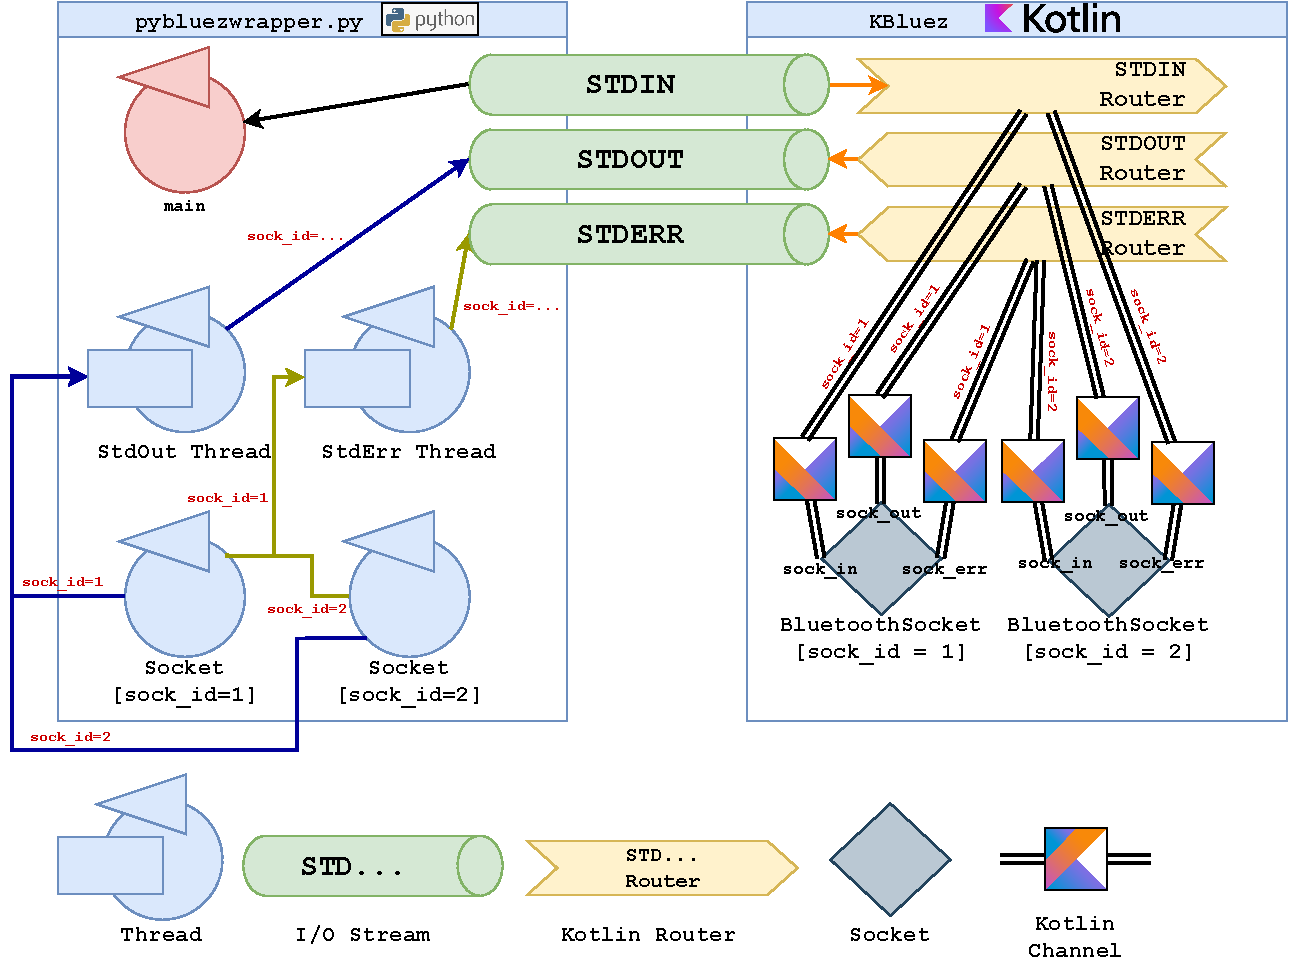
\includegraphics[width=\textwidth]{img/kbluez_general_architecture.pdf}
	\caption{General architecture of the \texttt{KBluez} library}
	\label{fig:kbluez_general_architecture}
\end{figure}

The figure \ref{fig:kbluez_general_architecture} shows a general overview of the architecture of our \texttt{KBluez}.

\begin{figure}[h!]
	\centering
	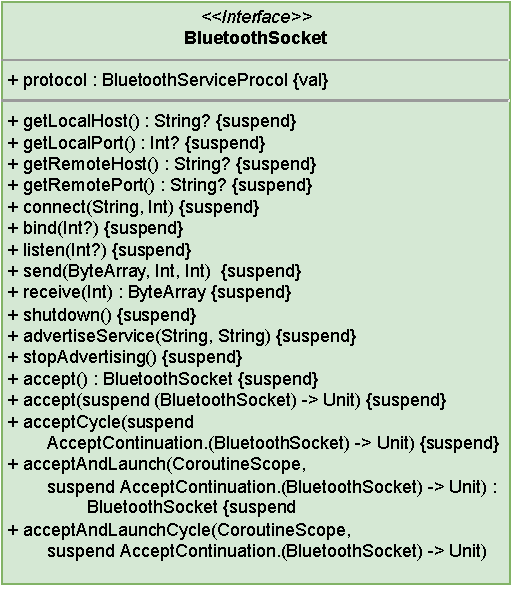
\includegraphics[width=0.4\textwidth]{img/uml_bluetooth_socket_interface.pdf}
	\caption{Class diagram of \texttt{it.unibo.kBluez.socket.BluetoothSocket}}
	\label{fig:uml_bluetooth_socket_interface}
\end{figure}

The figure \ref{fig:uml_bluetooth_socket_interface} shows the class diagram of the \texttt{BluetoothSocket} interface that is the main key point of our library. Other classes will not be shown at the moment.
This interface is implemented by \href{https://github.com/LM-96/MobileSystemProject/blob/main/kBluez/lib/src/main/kotlin/it/unibo/kBluez/pybluez/PyBluezSocket.kt}{PyBluezSocket} class but the implementation will not be exposed in deep.

At the operational point of view, the developer can obtain a \href{https://github.com/LM-96/MobileSystemProject/blob/main/kBluez/lib/src/main/kotlin/it/unibo/kBluez/socket/BluetoothSocket.kt}{\texttt{BluetoothSocket}} with \href{https://en.wikipedia.org/wiki/List_of_Bluetooth_protocols#Radio_frequency_communication_(RFCOMM)}{\texttt{RFCOMM}}by invoking:
\begin{lstlisting}[language=Kotlin]
	val btSock = KBLUEZ.requestNewSocket(BluetoothServiceProtocol.RFCOMM)
\end{lstlisting}
Then, this socket can be used exactly as the internet protocol sockets in order to build a client or a server.

\begin{tcolorbox}
	\begin{center}
		\textbf{We have used \texttt{BluetoothSocket} implementation in order to create a bluetooth server on \texttt{Raspberry} that make it able to communicate with the device of the user.}
	\end{center}
\end{tcolorbox}





